\begin{center}
    

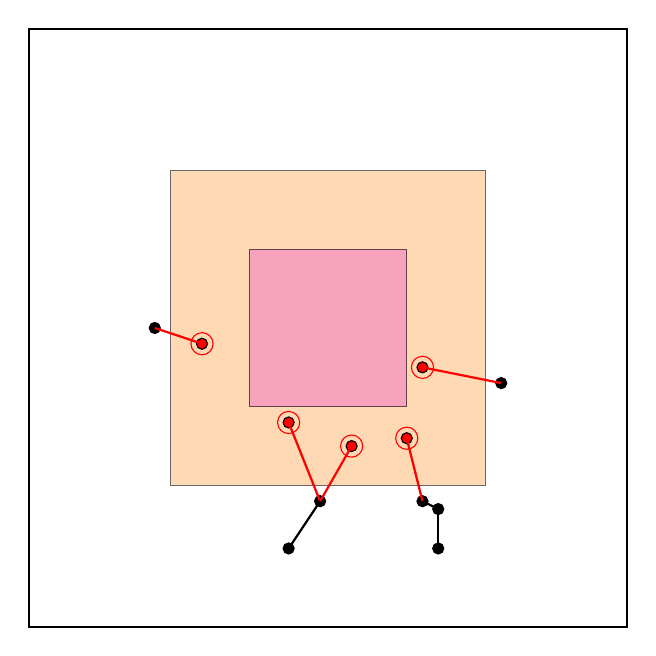
\begin{tikzpicture}

    % Square in the middle
    \draw[thick] (1.2, 1.2) rectangle ++(7.6, 7.6);
    \draw[fill=orange!50, opacity = 0.6] (3, 3) rectangle ++(4, 4);
    \draw[fill=magenta!50, opacity = 0.6] (4, 4) rectangle ++(2, 2);

    \coordinate (v1) at (2.8, 5);

    \filldraw[fill=black] (v1) circle (2pt);

    \coordinate (v6) at (4.9, 2.8);

    \filldraw[fill=black] (v6) circle (2pt);

    \coordinate (v72) at (4.5, 2.2);

    \filldraw[fill=black] (v72) circle (2pt);

    \coordinate (v9b) at (6.2, 2.8);

    \filldraw[fill=black] (v9b) circle (2pt);

    \coordinate (v9c) at (6.4, 2.7);

    \filldraw[fill=black] (v9c) circle (2pt);

    \coordinate (v9d) at (6.4, 2.2);

    \filldraw[fill=black] (v9d) circle (2pt);

    \coordinate (v92) at (7.2, 4.3);

    \filldraw[fill=black] (v92) circle (2pt);


    

    

    \coordinate (v2) at (3.4, 4.8);

    \filldraw[fill=red] (v2) circle (2pt);

    \draw[red] (v2) circle (4pt);

    \coordinate (v5) at (4.5, 3.8);

    \filldraw[fill=red] (v5) circle (2pt);

    \draw[red] (v5) circle (4pt);

    \coordinate (v71) at (5.3, 3.5);

    \filldraw[fill=red] (v71) circle (2pt);

    \draw[red] (v71) circle (4pt);

    \coordinate (v9a) at (6, 3.6);

    \filldraw[fill=red] (v9a) circle (2pt);

    \draw[red] (v9a) circle (4pt);

    \coordinate (v91) at (6.2, 4.5);

    \filldraw[fill=red] (v91) circle (2pt);

    \draw[red] (v91) circle (4pt);

    

    



    \draw [thick, red](v1) -- (v2);
    \draw [thick, red](v5) -- (v6);
    \draw [thick, red](v6) -- (v71);
    \draw [thick, red](v91) -- (v92);
    \draw [thick, red](v9a) -- (v9b);


    


    \draw [thick, black](v6) -- (v72);
    \draw [thick, black](v9b) -- (v9c);
    \draw [thick, black](v9c) -- (v9d);


   

    

\end{tikzpicture}

\end{center}